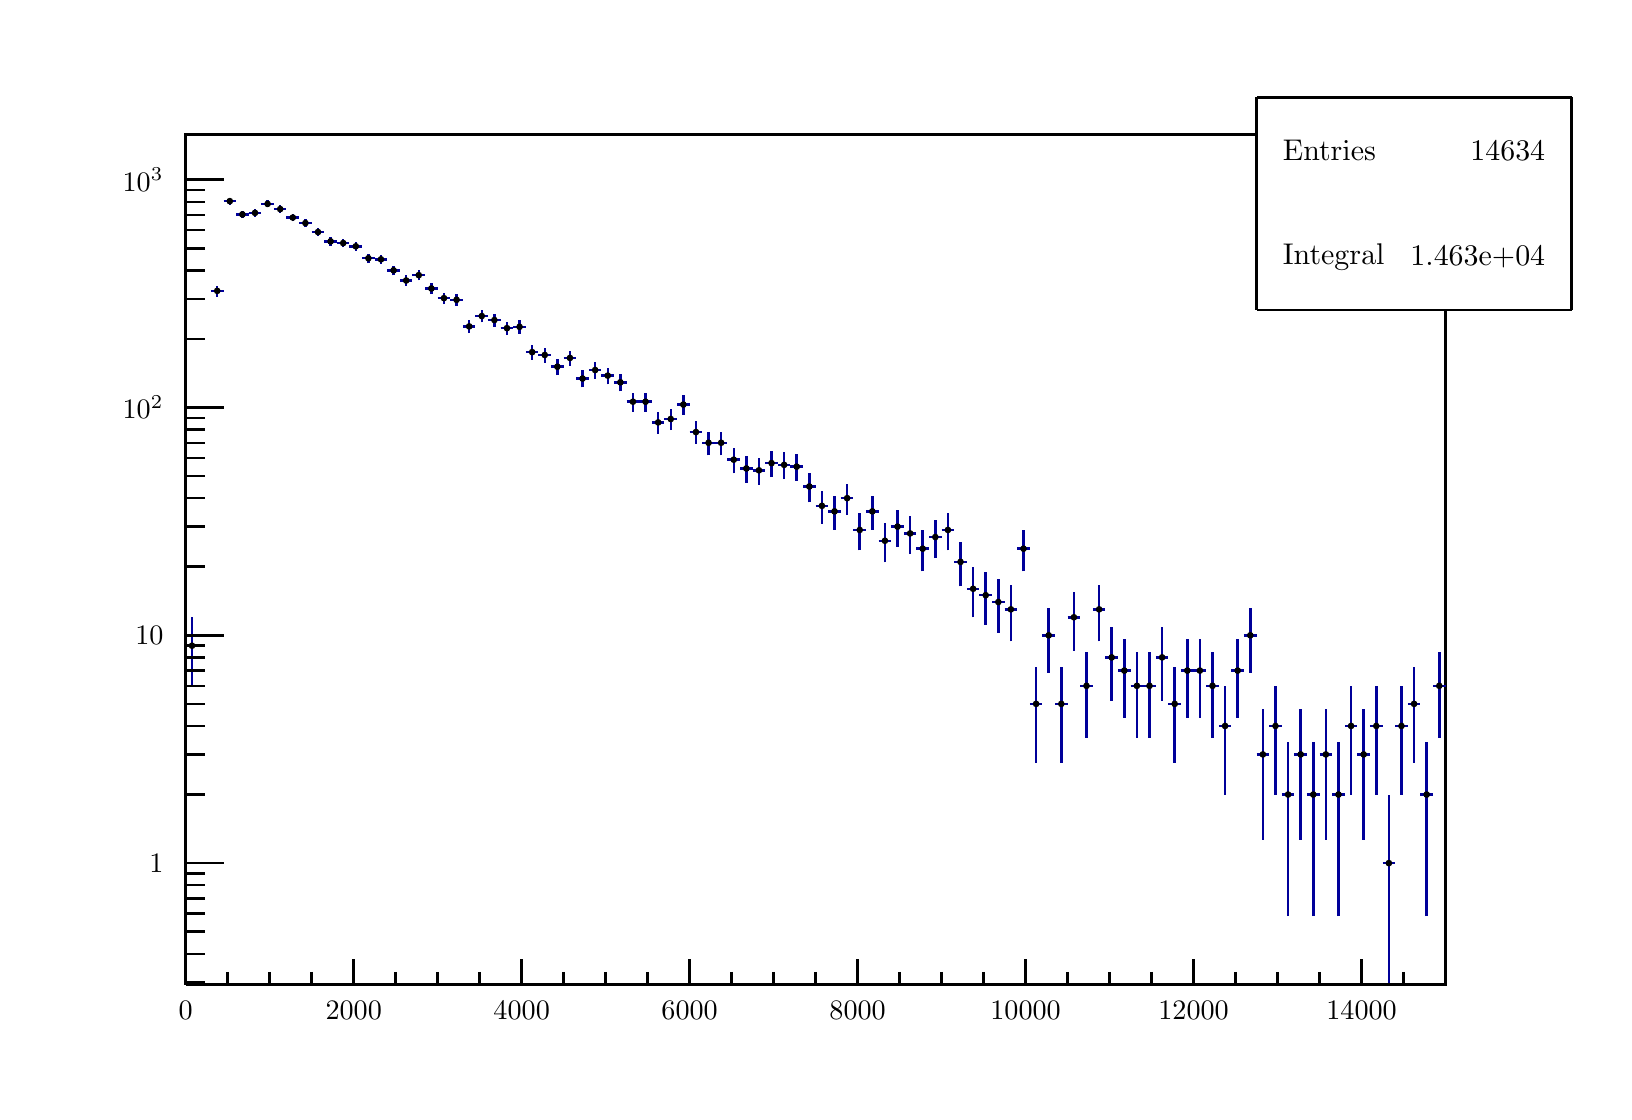
\begin{tikzpicture}
\pgfdeclareplotmark{cross} {
\pgfpathmoveto{\pgfpoint{-0.3\pgfplotmarksize}{\pgfplotmarksize}}
\pgfpathlineto{\pgfpoint{+0.3\pgfplotmarksize}{\pgfplotmarksize}}
\pgfpathlineto{\pgfpoint{+0.3\pgfplotmarksize}{0.3\pgfplotmarksize}}
\pgfpathlineto{\pgfpoint{+1\pgfplotmarksize}{0.3\pgfplotmarksize}}
\pgfpathlineto{\pgfpoint{+1\pgfplotmarksize}{-0.3\pgfplotmarksize}}
\pgfpathlineto{\pgfpoint{+0.3\pgfplotmarksize}{-0.3\pgfplotmarksize}}
\pgfpathlineto{\pgfpoint{+0.3\pgfplotmarksize}{-1.\pgfplotmarksize}}
\pgfpathlineto{\pgfpoint{-0.3\pgfplotmarksize}{-1.\pgfplotmarksize}}
\pgfpathlineto{\pgfpoint{-0.3\pgfplotmarksize}{-0.3\pgfplotmarksize}}
\pgfpathlineto{\pgfpoint{-1.\pgfplotmarksize}{-0.3\pgfplotmarksize}}
\pgfpathlineto{\pgfpoint{-1.\pgfplotmarksize}{0.3\pgfplotmarksize}}
\pgfpathlineto{\pgfpoint{-0.3\pgfplotmarksize}{0.3\pgfplotmarksize}}
\pgfpathclose
\pgfusepathqstroke
}
\pgfdeclareplotmark{cross*} {
\pgfpathmoveto{\pgfpoint{-0.3\pgfplotmarksize}{\pgfplotmarksize}}
\pgfpathlineto{\pgfpoint{+0.3\pgfplotmarksize}{\pgfplotmarksize}}
\pgfpathlineto{\pgfpoint{+0.3\pgfplotmarksize}{0.3\pgfplotmarksize}}
\pgfpathlineto{\pgfpoint{+1\pgfplotmarksize}{0.3\pgfplotmarksize}}
\pgfpathlineto{\pgfpoint{+1\pgfplotmarksize}{-0.3\pgfplotmarksize}}
\pgfpathlineto{\pgfpoint{+0.3\pgfplotmarksize}{-0.3\pgfplotmarksize}}
\pgfpathlineto{\pgfpoint{+0.3\pgfplotmarksize}{-1.\pgfplotmarksize}}
\pgfpathlineto{\pgfpoint{-0.3\pgfplotmarksize}{-1.\pgfplotmarksize}}
\pgfpathlineto{\pgfpoint{-0.3\pgfplotmarksize}{-0.3\pgfplotmarksize}}
\pgfpathlineto{\pgfpoint{-1.\pgfplotmarksize}{-0.3\pgfplotmarksize}}
\pgfpathlineto{\pgfpoint{-1.\pgfplotmarksize}{0.3\pgfplotmarksize}}
\pgfpathlineto{\pgfpoint{-0.3\pgfplotmarksize}{0.3\pgfplotmarksize}}
\pgfpathclose
\pgfusepathqfillstroke
}
\pgfdeclareplotmark{newstar} {
\pgfpathmoveto{\pgfqpoint{0pt}{\pgfplotmarksize}}
\pgfpathlineto{\pgfqpointpolar{44}{0.5\pgfplotmarksize}}
\pgfpathlineto{\pgfqpointpolar{18}{\pgfplotmarksize}}
\pgfpathlineto{\pgfqpointpolar{-20}{0.5\pgfplotmarksize}}
\pgfpathlineto{\pgfqpointpolar{-54}{\pgfplotmarksize}}
\pgfpathlineto{\pgfqpointpolar{-90}{0.5\pgfplotmarksize}}
\pgfpathlineto{\pgfqpointpolar{234}{\pgfplotmarksize}}
\pgfpathlineto{\pgfqpointpolar{198}{0.5\pgfplotmarksize}}
\pgfpathlineto{\pgfqpointpolar{162}{\pgfplotmarksize}}
\pgfpathlineto{\pgfqpointpolar{134}{0.5\pgfplotmarksize}}
\pgfpathclose
\pgfusepathqstroke
}
\pgfdeclareplotmark{newstar*} {
\pgfpathmoveto{\pgfqpoint{0pt}{\pgfplotmarksize}}
\pgfpathlineto{\pgfqpointpolar{44}{0.5\pgfplotmarksize}}
\pgfpathlineto{\pgfqpointpolar{18}{\pgfplotmarksize}}
\pgfpathlineto{\pgfqpointpolar{-20}{0.5\pgfplotmarksize}}
\pgfpathlineto{\pgfqpointpolar{-54}{\pgfplotmarksize}}
\pgfpathlineto{\pgfqpointpolar{-90}{0.5\pgfplotmarksize}}
\pgfpathlineto{\pgfqpointpolar{234}{\pgfplotmarksize}}
\pgfpathlineto{\pgfqpointpolar{198}{0.5\pgfplotmarksize}}
\pgfpathlineto{\pgfqpointpolar{162}{\pgfplotmarksize}}
\pgfpathlineto{\pgfqpointpolar{134}{0.5\pgfplotmarksize}}
\pgfpathclose
\pgfusepathqfillstroke
}
\definecolor{c}{rgb}{1,1,1};
\draw [color=c, fill=c] (0,0) rectangle (20,13.4957);
\draw [color=c, fill=c] (2,1.34957) rectangle (18,12.1461);
\definecolor{c}{rgb}{0,0,0};
\draw [c,line width=0.9] (2,1.34957) -- (2,12.1461) -- (18,12.1461) -- (18,1.34957) -- (2,1.34957);
\definecolor{c}{rgb}{1,1,1};
\draw [color=c, fill=c] (2,1.34957) rectangle (18,12.1461);
\definecolor{c}{rgb}{0,0,0};
\draw [c,line width=0.9] (2,1.34957) -- (2,12.1461) -- (18,12.1461) -- (18,1.34957) -- (2,1.34957);
\definecolor{c}{rgb}{0,0,0.6};
\draw [c,line width=0.9] (2.08,5.14386) -- (2.08,5.65333);
\draw [c,line width=0.9] (2.08,5.65333) -- (2.08,6.0148);
\draw [c,line width=0.9] (2,5.65333) -- (2.08,5.65333);
\draw [c,line width=0.9] (2.08,5.65333) -- (2.16,5.65333);
\definecolor{c}{rgb}{0,0,0};
\foreach \P in {(2.08,5.65333)}{\draw[mark options={color=c,fill=c},mark size=2.402402pt,mark=*,mark size=1pt] plot coordinates {\P};}
\definecolor{c}{rgb}{0,0,0.6};
\draw [c,line width=0.9] (2.4,10.0882) -- (2.4,10.1599);
\draw [c,line width=0.9] (2.4,10.1599) -- (2.4,10.2278);
\draw [c,line width=0.9] (2.32,10.1599) -- (2.4,10.1599);
\draw [c,line width=0.9] (2.4,10.1599) -- (2.48,10.1599);
\definecolor{c}{rgb}{0,0,0};
\foreach \P in {(2.4,10.1599)}{\draw[mark options={color=c,fill=c},mark size=2.402402pt,mark=*,mark size=1pt] plot coordinates {\P};}
\definecolor{c}{rgb}{0,0,0.6};
\draw [c,line width=0.9] (2.56,11.2545) -- (2.56,11.2996);
\draw [c,line width=0.9] (2.56,11.2996) -- (2.56,11.3431);
\draw [c,line width=0.9] (2.48,11.2996) -- (2.56,11.2996);
\draw [c,line width=0.9] (2.56,11.2996) -- (2.64,11.2996);
\definecolor{c}{rgb}{0,0,0};
\foreach \P in {(2.56,11.2996)}{\draw[mark options={color=c,fill=c},mark size=2.402402pt,mark=*,mark size=1pt] plot coordinates {\P};}
\definecolor{c}{rgb}{0,0,0.6};
\draw [c,line width=0.9] (2.72,11.0829) -- (2.72,11.1311);
\draw [c,line width=0.9] (2.72,11.1311) -- (2.72,11.1776);
\draw [c,line width=0.9] (2.64,11.1311) -- (2.72,11.1311);
\draw [c,line width=0.9] (2.72,11.1311) -- (2.8,11.1311);
\definecolor{c}{rgb}{0,0,0};
\foreach \P in {(2.72,11.1311)}{\draw[mark options={color=c,fill=c},mark size=2.402402pt,mark=*,mark size=1pt] plot coordinates {\P};}
\definecolor{c}{rgb}{0,0,0.6};
\draw [c,line width=0.9] (2.88,11.1027) -- (2.88,11.1506);
\draw [c,line width=0.9] (2.88,11.1506) -- (2.88,11.1968);
\draw [c,line width=0.9] (2.8,11.1506) -- (2.88,11.1506);
\draw [c,line width=0.9] (2.88,11.1506) -- (2.96,11.1506);
\definecolor{c}{rgb}{0,0,0};
\foreach \P in {(2.88,11.1506)}{\draw[mark options={color=c,fill=c},mark size=2.402402pt,mark=*,mark size=1pt] plot coordinates {\P};}
\definecolor{c}{rgb}{0,0,0.6};
\draw [c,line width=0.9] (3.04,11.2191) -- (3.04,11.2648);
\draw [c,line width=0.9] (3.04,11.2648) -- (3.04,11.3089);
\draw [c,line width=0.9] (2.96,11.2648) -- (3.04,11.2648);
\draw [c,line width=0.9] (3.04,11.2648) -- (3.12,11.2648);
\definecolor{c}{rgb}{0,0,0};
\foreach \P in {(3.04,11.2648)}{\draw[mark options={color=c,fill=c},mark size=2.402402pt,mark=*,mark size=1pt] plot coordinates {\P};}
\definecolor{c}{rgb}{0,0,0.6};
\draw [c,line width=0.9] (3.2,11.1519) -- (3.2,11.1989);
\draw [c,line width=0.9] (3.2,11.1989) -- (3.2,11.2442);
\draw [c,line width=0.9] (3.12,11.1989) -- (3.2,11.1989);
\draw [c,line width=0.9] (3.2,11.1989) -- (3.28,11.1989);
\definecolor{c}{rgb}{0,0,0};
\foreach \P in {(3.2,11.1989)}{\draw[mark options={color=c,fill=c},mark size=2.402402pt,mark=*,mark size=1pt] plot coordinates {\P};}
\definecolor{c}{rgb}{0,0,0.6};
\draw [c,line width=0.9] (3.36,11.0422) -- (3.36,11.0913);
\draw [c,line width=0.9] (3.36,11.0913) -- (3.36,11.1385);
\draw [c,line width=0.9] (3.28,11.0913) -- (3.36,11.0913);
\draw [c,line width=0.9] (3.36,11.0913) -- (3.44,11.0913);
\definecolor{c}{rgb}{0,0,0};
\foreach \P in {(3.36,11.0913)}{\draw[mark options={color=c,fill=c},mark size=2.402402pt,mark=*,mark size=1pt] plot coordinates {\P};}
\definecolor{c}{rgb}{0,0,0.6};
\draw [c,line width=0.9] (3.52,10.9707) -- (3.52,11.0212);
\draw [c,line width=0.9] (3.52,11.0212) -- (3.52,11.0697);
\draw [c,line width=0.9] (3.44,11.0212) -- (3.52,11.0212);
\draw [c,line width=0.9] (3.52,11.0212) -- (3.6,11.0212);
\definecolor{c}{rgb}{0,0,0};
\foreach \P in {(3.52,11.0212)}{\draw[mark options={color=c,fill=c},mark size=2.402402pt,mark=*,mark size=1pt] plot coordinates {\P};}
\definecolor{c}{rgb}{0,0,0.6};
\draw [c,line width=0.9] (3.68,10.8542) -- (3.68,10.907);
\draw [c,line width=0.9] (3.68,10.907) -- (3.68,10.9578);
\draw [c,line width=0.9] (3.6,10.907) -- (3.68,10.907);
\draw [c,line width=0.9] (3.68,10.907) -- (3.76,10.907);
\definecolor{c}{rgb}{0,0,0};
\foreach \P in {(3.68,10.907)}{\draw[mark options={color=c,fill=c},mark size=2.402402pt,mark=*,mark size=1pt] plot coordinates {\P};}
\definecolor{c}{rgb}{0,0,0.6};
\draw [c,line width=0.9] (3.84,10.7331) -- (3.84,10.7886);
\draw [c,line width=0.9] (3.84,10.7886) -- (3.84,10.8417);
\draw [c,line width=0.9] (3.76,10.7886) -- (3.84,10.7886);
\draw [c,line width=0.9] (3.84,10.7886) -- (3.92,10.7886);
\definecolor{c}{rgb}{0,0,0};
\foreach \P in {(3.84,10.7886)}{\draw[mark options={color=c,fill=c},mark size=2.402402pt,mark=*,mark size=1pt] plot coordinates {\P};}
\definecolor{c}{rgb}{0,0,0.6};
\draw [c,line width=0.9] (4,10.7113) -- (4,10.7673);
\draw [c,line width=0.9] (4,10.7673) -- (4,10.8209);
\draw [c,line width=0.9] (3.92,10.7673) -- (4,10.7673);
\draw [c,line width=0.9] (4,10.7673) -- (4.08,10.7673);
\definecolor{c}{rgb}{0,0,0};
\foreach \P in {(4,10.7673)}{\draw[mark options={color=c,fill=c},mark size=2.402402pt,mark=*,mark size=1pt] plot coordinates {\P};}
\definecolor{c}{rgb}{0,0,0.6};
\draw [c,line width=0.9] (4.16,10.6692) -- (4.16,10.7261);
\draw [c,line width=0.9] (4.16,10.7261) -- (4.16,10.7805);
\draw [c,line width=0.9] (4.08,10.7261) -- (4.16,10.7261);
\draw [c,line width=0.9] (4.16,10.7261) -- (4.24,10.7261);
\definecolor{c}{rgb}{0,0,0};
\foreach \P in {(4.16,10.7261)}{\draw[mark options={color=c,fill=c},mark size=2.402402pt,mark=*,mark size=1pt] plot coordinates {\P};}
\definecolor{c}{rgb}{0,0,0.6};
\draw [c,line width=0.9] (4.32,10.5139) -- (4.32,10.5744);
\draw [c,line width=0.9] (4.32,10.5744) -- (4.32,10.6321);
\draw [c,line width=0.9] (4.24,10.5744) -- (4.32,10.5744);
\draw [c,line width=0.9] (4.32,10.5744) -- (4.4,10.5744);
\definecolor{c}{rgb}{0,0,0};
\foreach \P in {(4.32,10.5744)}{\draw[mark options={color=c,fill=c},mark size=2.402402pt,mark=*,mark size=1pt] plot coordinates {\P};}
\definecolor{c}{rgb}{0,0,0.6};
\draw [c,line width=0.9] (4.48,10.4995) -- (4.48,10.5604);
\draw [c,line width=0.9] (4.48,10.5604) -- (4.48,10.6185);
\draw [c,line width=0.9] (4.4,10.5604) -- (4.48,10.5604);
\draw [c,line width=0.9] (4.48,10.5604) -- (4.56,10.5604);
\definecolor{c}{rgb}{0,0,0};
\foreach \P in {(4.48,10.5604)}{\draw[mark options={color=c,fill=c},mark size=2.402402pt,mark=*,mark size=1pt] plot coordinates {\P};}
\definecolor{c}{rgb}{0,0,0.6};
\draw [c,line width=0.9] (4.64,10.3564) -- (4.64,10.4208);
\draw [c,line width=0.9] (4.64,10.4208) -- (4.64,10.4821);
\draw [c,line width=0.9] (4.56,10.4208) -- (4.64,10.4208);
\draw [c,line width=0.9] (4.64,10.4208) -- (4.72,10.4208);
\definecolor{c}{rgb}{0,0,0};
\foreach \P in {(4.64,10.4208)}{\draw[mark options={color=c,fill=c},mark size=2.402402pt,mark=*,mark size=1pt] plot coordinates {\P};}
\definecolor{c}{rgb}{0,0,0.6};
\draw [c,line width=0.9] (4.8,10.224) -- (4.8,10.2919);
\draw [c,line width=0.9] (4.8,10.2919) -- (4.8,10.3564);
\draw [c,line width=0.9] (4.72,10.2919) -- (4.8,10.2919);
\draw [c,line width=0.9] (4.8,10.2919) -- (4.88,10.2919);
\definecolor{c}{rgb}{0,0,0};
\foreach \P in {(4.8,10.2919)}{\draw[mark options={color=c,fill=c},mark size=2.402402pt,mark=*,mark size=1pt] plot coordinates {\P};}
\definecolor{c}{rgb}{0,0,0.6};
\draw [c,line width=0.9] (4.96,10.2936) -- (4.96,10.3597);
\draw [c,line width=0.9] (4.96,10.3597) -- (4.96,10.4225);
\draw [c,line width=0.9] (4.88,10.3597) -- (4.96,10.3597);
\draw [c,line width=0.9] (4.96,10.3597) -- (5.04,10.3597);
\definecolor{c}{rgb}{0,0,0};
\foreach \P in {(4.96,10.3597)}{\draw[mark options={color=c,fill=c},mark size=2.402402pt,mark=*,mark size=1pt] plot coordinates {\P};}
\definecolor{c}{rgb}{0,0,0.6};
\draw [c,line width=0.9] (5.12,10.1197) -- (5.12,10.1905);
\draw [c,line width=0.9] (5.12,10.1905) -- (5.12,10.2575);
\draw [c,line width=0.9] (5.04,10.1905) -- (5.12,10.1905);
\draw [c,line width=0.9] (5.12,10.1905) -- (5.2,10.1905);
\definecolor{c}{rgb}{0,0,0};
\foreach \P in {(5.12,10.1905)}{\draw[mark options={color=c,fill=c},mark size=2.402402pt,mark=*,mark size=1pt] plot coordinates {\P};}
\definecolor{c}{rgb}{0,0,0.6};
\draw [c,line width=0.9] (5.28,9.99323) -- (5.28,10.0677);
\draw [c,line width=0.9] (5.28,10.0677) -- (5.28,10.138);
\draw [c,line width=0.9] (5.2,10.0677) -- (5.28,10.0677);
\draw [c,line width=0.9] (5.28,10.0677) -- (5.36,10.0677);
\definecolor{c}{rgb}{0,0,0};
\foreach \P in {(5.28,10.0677)}{\draw[mark options={color=c,fill=c},mark size=2.402402pt,mark=*,mark size=1pt] plot coordinates {\P};}
\definecolor{c}{rgb}{0,0,0.6};
\draw [c,line width=0.9] (5.44,9.97161) -- (5.44,10.0467);
\draw [c,line width=0.9] (5.44,10.0467) -- (5.44,10.1176);
\draw [c,line width=0.9] (5.36,10.0467) -- (5.44,10.0467);
\draw [c,line width=0.9] (5.44,10.0467) -- (5.52,10.0467);
\definecolor{c}{rgb}{0,0,0};
\foreach \P in {(5.44,10.0467)}{\draw[mark options={color=c,fill=c},mark size=2.402402pt,mark=*,mark size=1pt] plot coordinates {\P};}
\definecolor{c}{rgb}{0,0,0.6};
\draw [c,line width=0.9] (5.6,9.6227) -- (5.6,9.70899);
\draw [c,line width=0.9] (5.6,9.70899) -- (5.6,9.78974);
\draw [c,line width=0.9] (5.52,9.70899) -- (5.6,9.70899);
\draw [c,line width=0.9] (5.6,9.70899) -- (5.68,9.70899);
\definecolor{c}{rgb}{0,0,0};
\foreach \P in {(5.6,9.70899)}{\draw[mark options={color=c,fill=c},mark size=2.402402pt,mark=*,mark size=1pt] plot coordinates {\P};}
\definecolor{c}{rgb}{0,0,0.6};
\draw [c,line width=0.9] (5.76,9.75852) -- (5.76,9.84027);
\draw [c,line width=0.9] (5.76,9.84027) -- (5.76,9.91703);
\draw [c,line width=0.9] (5.68,9.84027) -- (5.76,9.84027);
\draw [c,line width=0.9] (5.76,9.84027) -- (5.84,9.84027);
\definecolor{c}{rgb}{0,0,0};
\foreach \P in {(5.76,9.84027)}{\draw[mark options={color=c,fill=c},mark size=2.402402pt,mark=*,mark size=1pt] plot coordinates {\P};}
\definecolor{c}{rgb}{0,0,0.6};
\draw [c,line width=0.9] (5.92,9.70591) -- (5.92,9.7894);
\draw [c,line width=0.9] (5.92,9.7894) -- (5.92,9.86768);
\draw [c,line width=0.9] (5.84,9.7894) -- (5.92,9.7894);
\draw [c,line width=0.9] (5.92,9.7894) -- (6,9.7894);
\definecolor{c}{rgb}{0,0,0};
\foreach \P in {(5.92,9.7894)}{\draw[mark options={color=c,fill=c},mark size=2.402402pt,mark=*,mark size=1pt] plot coordinates {\P};}
\definecolor{c}{rgb}{0,0,0.6};
\draw [c,line width=0.9] (6.08,9.59956) -- (6.08,9.68666);
\draw [c,line width=0.9] (6.08,9.68666) -- (6.08,9.7681);
\draw [c,line width=0.9] (6,9.68666) -- (6.08,9.68666);
\draw [c,line width=0.9] (6.08,9.68666) -- (6.16,9.68666);
\definecolor{c}{rgb}{0,0,0};
\foreach \P in {(6.08,9.68666)}{\draw[mark options={color=c,fill=c},mark size=2.402402pt,mark=*,mark size=1pt] plot coordinates {\P};}
\definecolor{c}{rgb}{0,0,0.6};
\draw [c,line width=0.9] (6.24,9.61695) -- (6.24,9.70345);
\draw [c,line width=0.9] (6.24,9.70345) -- (6.24,9.78437);
\draw [c,line width=0.9] (6.16,9.70345) -- (6.24,9.70345);
\draw [c,line width=0.9] (6.24,9.70345) -- (6.32,9.70345);
\definecolor{c}{rgb}{0,0,0};
\foreach \P in {(6.24,9.70345)}{\draw[mark options={color=c,fill=c},mark size=2.402402pt,mark=*,mark size=1pt] plot coordinates {\P};}
\definecolor{c}{rgb}{0,0,0.6};
\draw [c,line width=0.9] (6.4,9.28333) -- (6.4,9.3821);
\draw [c,line width=0.9] (6.4,9.3821) -- (6.4,9.47366);
\draw [c,line width=0.9] (6.32,9.3821) -- (6.4,9.3821);
\draw [c,line width=0.9] (6.4,9.3821) -- (6.48,9.3821);
\definecolor{c}{rgb}{0,0,0};
\foreach \P in {(6.4,9.3821)}{\draw[mark options={color=c,fill=c},mark size=2.402402pt,mark=*,mark size=1pt] plot coordinates {\P};}
\definecolor{c}{rgb}{0,0,0.6};
\draw [c,line width=0.9] (6.56,9.24541) -- (6.56,9.34567);
\draw [c,line width=0.9] (6.56,9.34567) -- (6.56,9.43853);
\draw [c,line width=0.9] (6.48,9.34567) -- (6.56,9.34567);
\draw [c,line width=0.9] (6.56,9.34567) -- (6.64,9.34567);
\definecolor{c}{rgb}{0,0,0};
\foreach \P in {(6.56,9.34567)}{\draw[mark options={color=c,fill=c},mark size=2.402402pt,mark=*,mark size=1pt] plot coordinates {\P};}
\definecolor{c}{rgb}{0,0,0.6};
\draw [c,line width=0.9] (6.72,9.0901) -- (6.72,9.19675);
\draw [c,line width=0.9] (6.72,9.19675) -- (6.72,9.29506);
\draw [c,line width=0.9] (6.64,9.19675) -- (6.72,9.19675);
\draw [c,line width=0.9] (6.72,9.19675) -- (6.8,9.19675);
\definecolor{c}{rgb}{0,0,0};
\foreach \P in {(6.72,9.19675)}{\draw[mark options={color=c,fill=c},mark size=2.402402pt,mark=*,mark size=1pt] plot coordinates {\P};}
\definecolor{c}{rgb}{0,0,0.6};
\draw [c,line width=0.9] (6.88,9.20633) -- (6.88,9.30816);
\draw [c,line width=0.9] (6.88,9.30816) -- (6.88,9.40236);
\draw [c,line width=0.9] (6.8,9.30816) -- (6.88,9.30816);
\draw [c,line width=0.9] (6.88,9.30816) -- (6.96,9.30816);
\definecolor{c}{rgb}{0,0,0};
\foreach \P in {(6.88,9.30816)}{\draw[mark options={color=c,fill=c},mark size=2.402402pt,mark=*,mark size=1pt] plot coordinates {\P};}
\definecolor{c}{rgb}{0,0,0.6};
\draw [c,line width=0.9] (7.04,8.93315) -- (7.04,9.04667);
\draw [c,line width=0.9] (7.04,9.04667) -- (7.04,9.15079);
\draw [c,line width=0.9] (6.96,9.04667) -- (7.04,9.04667);
\draw [c,line width=0.9] (7.04,9.04667) -- (7.12,9.04667);
\definecolor{c}{rgb}{0,0,0};
\foreach \P in {(7.04,9.04667)}{\draw[mark options={color=c,fill=c},mark size=2.402402pt,mark=*,mark size=1pt] plot coordinates {\P};}
\definecolor{c}{rgb}{0,0,0.6};
\draw [c,line width=0.9] (7.2,9.0459) -- (7.2,9.15444);
\draw [c,line width=0.9] (7.2,9.15444) -- (7.2,9.25435);
\draw [c,line width=0.9] (7.12,9.15444) -- (7.2,9.15444);
\draw [c,line width=0.9] (7.2,9.15444) -- (7.28,9.15444);
\definecolor{c}{rgb}{0,0,0};
\foreach \P in {(7.2,9.15444)}{\draw[mark options={color=c,fill=c},mark size=2.402402pt,mark=*,mark size=1pt] plot coordinates {\P};}
\definecolor{c}{rgb}{0,0,0.6};
\draw [c,line width=0.9] (7.36,8.97184) -- (7.36,9.08363);
\draw [c,line width=0.9] (7.36,9.08363) -- (7.36,9.18629);
\draw [c,line width=0.9] (7.28,9.08363) -- (7.36,9.08363);
\draw [c,line width=0.9] (7.36,9.08363) -- (7.44,9.08363);
\definecolor{c}{rgb}{0,0,0};
\foreach \P in {(7.36,9.08363)}{\draw[mark options={color=c,fill=c},mark size=2.402402pt,mark=*,mark size=1pt] plot coordinates {\P};}
\definecolor{c}{rgb}{0,0,0.6};
\draw [c,line width=0.9] (7.52,8.88309) -- (7.52,8.99889);
\draw [c,line width=0.9] (7.52,8.99889) -- (7.52,9.10492);
\draw [c,line width=0.9] (7.44,8.99889) -- (7.52,8.99889);
\draw [c,line width=0.9] (7.52,8.99889) -- (7.6,8.99889);
\definecolor{c}{rgb}{0,0,0};
\foreach \P in {(7.52,8.99889)}{\draw[mark options={color=c,fill=c},mark size=2.402402pt,mark=*,mark size=1pt] plot coordinates {\P};}
\definecolor{c}{rgb}{0,0,0.6};
\draw [c,line width=0.9] (7.68,8.62376) -- (7.68,8.75215);
\draw [c,line width=0.9] (7.68,8.75215) -- (7.68,8.86862);
\draw [c,line width=0.9] (7.6,8.75215) -- (7.68,8.75215);
\draw [c,line width=0.9] (7.68,8.75215) -- (7.76,8.75215);
\definecolor{c}{rgb}{0,0,0};
\foreach \P in {(7.68,8.75215)}{\draw[mark options={color=c,fill=c},mark size=2.402402pt,mark=*,mark size=1pt] plot coordinates {\P};}
\definecolor{c}{rgb}{0,0,0.6};
\draw [c,line width=0.9] (7.84,8.62376) -- (7.84,8.75215);
\draw [c,line width=0.9] (7.84,8.75215) -- (7.84,8.86862);
\draw [c,line width=0.9] (7.76,8.75215) -- (7.84,8.75215);
\draw [c,line width=0.9] (7.84,8.75215) -- (7.92,8.75215);
\definecolor{c}{rgb}{0,0,0};
\foreach \P in {(7.84,8.75215)}{\draw[mark options={color=c,fill=c},mark size=2.402402pt,mark=*,mark size=1pt] plot coordinates {\P};}
\definecolor{c}{rgb}{0,0,0.6};
\draw [c,line width=0.9] (8,8.34605) -- (8,8.48942);
\draw [c,line width=0.9] (8,8.48942) -- (8,8.6181);
\draw [c,line width=0.9] (7.92,8.48942) -- (8,8.48942);
\draw [c,line width=0.9] (8,8.48942) -- (8.08,8.48942);
\definecolor{c}{rgb}{0,0,0};
\foreach \P in {(8,8.48942)}{\draw[mark options={color=c,fill=c},mark size=2.402402pt,mark=*,mark size=1pt] plot coordinates {\P};}
\definecolor{c}{rgb}{0,0,0.6};
\draw [c,line width=0.9] (8.16,8.39172) -- (8.16,8.53251);
\draw [c,line width=0.9] (8.16,8.53251) -- (8.16,8.6591);
\draw [c,line width=0.9] (8.08,8.53251) -- (8.16,8.53251);
\draw [c,line width=0.9] (8.16,8.53251) -- (8.24,8.53251);
\definecolor{c}{rgb}{0,0,0};
\foreach \P in {(8.16,8.53251)}{\draw[mark options={color=c,fill=c},mark size=2.402402pt,mark=*,mark size=1pt] plot coordinates {\P};}
\definecolor{c}{rgb}{0,0,0.6};
\draw [c,line width=0.9] (8.32,8.58573) -- (8.32,8.71607);
\draw [c,line width=0.9] (8.32,8.71607) -- (8.32,8.83416);
\draw [c,line width=0.9] (8.24,8.71607) -- (8.32,8.71607);
\draw [c,line width=0.9] (8.32,8.71607) -- (8.4,8.71607);
\definecolor{c}{rgb}{0,0,0};
\foreach \P in {(8.32,8.71607)}{\draw[mark options={color=c,fill=c},mark size=2.402402pt,mark=*,mark size=1pt] plot coordinates {\P};}
\definecolor{c}{rgb}{0,0,0.6};
\draw [c,line width=0.9] (8.48,8.21575) -- (8.48,8.36674);
\draw [c,line width=0.9] (8.48,8.36674) -- (8.48,8.50152);
\draw [c,line width=0.9] (8.4,8.36674) -- (8.48,8.36674);
\draw [c,line width=0.9] (8.48,8.36674) -- (8.56,8.36674);
\definecolor{c}{rgb}{0,0,0};
\foreach \P in {(8.48,8.36674)}{\draw[mark options={color=c,fill=c},mark size=2.402402pt,mark=*,mark size=1pt] plot coordinates {\P};}
\definecolor{c}{rgb}{0,0,0.6};
\draw [c,line width=0.9] (8.64,8.07083) -- (8.64,8.23077);
\draw [c,line width=0.9] (8.64,8.23077) -- (8.64,8.37263);
\draw [c,line width=0.9] (8.56,8.23077) -- (8.64,8.23077);
\draw [c,line width=0.9] (8.64,8.23077) -- (8.72,8.23077);
\definecolor{c}{rgb}{0,0,0};
\foreach \P in {(8.64,8.23077)}{\draw[mark options={color=c,fill=c},mark size=2.402402pt,mark=*,mark size=1pt] plot coordinates {\P};}
\definecolor{c}{rgb}{0,0,0.6};
\draw [c,line width=0.9] (8.8,8.07083) -- (8.8,8.23077);
\draw [c,line width=0.9] (8.8,8.23077) -- (8.8,8.37263);
\draw [c,line width=0.9] (8.72,8.23077) -- (8.8,8.23077);
\draw [c,line width=0.9] (8.8,8.23077) -- (8.88,8.23077);
\definecolor{c}{rgb}{0,0,0};
\foreach \P in {(8.8,8.23077)}{\draw[mark options={color=c,fill=c},mark size=2.402402pt,mark=*,mark size=1pt] plot coordinates {\P};}
\definecolor{c}{rgb}{0,0,0.6};
\draw [c,line width=0.9] (8.96,7.8407) -- (8.96,8.01596);
\draw [c,line width=0.9] (8.96,8.01596) -- (8.96,8.16974);
\draw [c,line width=0.9] (8.88,8.01596) -- (8.96,8.01596);
\draw [c,line width=0.9] (8.96,8.01596) -- (9.04,8.01596);
\definecolor{c}{rgb}{0,0,0};
\foreach \P in {(8.96,8.01596)}{\draw[mark options={color=c,fill=c},mark size=2.402402pt,mark=*,mark size=1pt] plot coordinates {\P};}
\definecolor{c}{rgb}{0,0,0.6};
\draw [c,line width=0.9] (9.12,7.72089) -- (9.12,7.90469);
\draw [c,line width=0.9] (9.12,7.90469) -- (9.12,8.065);
\draw [c,line width=0.9] (9.04,7.90469) -- (9.12,7.90469);
\draw [c,line width=0.9] (9.12,7.90469) -- (9.2,7.90469);
\definecolor{c}{rgb}{0,0,0};
\foreach \P in {(9.12,7.90469)}{\draw[mark options={color=c,fill=c},mark size=2.402402pt,mark=*,mark size=1pt] plot coordinates {\P};}
\definecolor{c}{rgb}{0,0,0.6};
\draw [c,line width=0.9] (9.28,7.69554) -- (9.28,7.8812);
\draw [c,line width=0.9] (9.28,7.8812) -- (9.28,8.04293);
\draw [c,line width=0.9] (9.2,7.8812) -- (9.28,7.8812);
\draw [c,line width=0.9] (9.28,7.8812) -- (9.36,7.8812);
\definecolor{c}{rgb}{0,0,0};
\foreach \P in {(9.28,7.8812)}{\draw[mark options={color=c,fill=c},mark size=2.402402pt,mark=*,mark size=1pt] plot coordinates {\P};}
\definecolor{c}{rgb}{0,0,0.6};
\draw [c,line width=0.9] (9.44,7.79409) -- (9.44,7.97263);
\draw [c,line width=0.9] (9.44,7.97263) -- (9.44,8.12892);
\draw [c,line width=0.9] (9.36,7.97263) -- (9.44,7.97263);
\draw [c,line width=0.9] (9.44,7.97263) -- (9.52,7.97263);
\definecolor{c}{rgb}{0,0,0};
\foreach \P in {(9.44,7.97263)}{\draw[mark options={color=c,fill=c},mark size=2.402402pt,mark=*,mark size=1pt] plot coordinates {\P};}
\definecolor{c}{rgb}{0,0,0.6};
\draw [c,line width=0.9] (9.6,7.77015) -- (9.6,7.95039);
\draw [c,line width=0.9] (9.6,7.95039) -- (9.6,8.10798);
\draw [c,line width=0.9] (9.52,7.95039) -- (9.6,7.95039);
\draw [c,line width=0.9] (9.6,7.95039) -- (9.68,7.95039);
\definecolor{c}{rgb}{0,0,0};
\foreach \P in {(9.6,7.95039)}{\draw[mark options={color=c,fill=c},mark size=2.402402pt,mark=*,mark size=1pt] plot coordinates {\P};}
\definecolor{c}{rgb}{0,0,0.6};
\draw [c,line width=0.9] (9.76,7.74575) -- (9.76,7.92775);
\draw [c,line width=0.9] (9.76,7.92775) -- (9.76,8.08668);
\draw [c,line width=0.9] (9.68,7.92775) -- (9.76,7.92775);
\draw [c,line width=0.9] (9.76,7.92775) -- (9.84,7.92775);
\definecolor{c}{rgb}{0,0,0};
\foreach \P in {(9.76,7.92775)}{\draw[mark options={color=c,fill=c},mark size=2.402402pt,mark=*,mark size=1pt] plot coordinates {\P};}
\definecolor{c}{rgb}{0,0,0.6};
\draw [c,line width=0.9] (9.92,7.47277) -- (9.92,7.6756);
\draw [c,line width=0.9] (9.92,7.6756) -- (9.92,7.8502);
\draw [c,line width=0.9] (9.84,7.6756) -- (9.92,7.6756);
\draw [c,line width=0.9] (9.92,7.6756) -- (10,7.6756);
\definecolor{c}{rgb}{0,0,0};
\foreach \P in {(9.92,7.6756)}{\draw[mark options={color=c,fill=c},mark size=2.402402pt,mark=*,mark size=1pt] plot coordinates {\P};}
\definecolor{c}{rgb}{0,0,0.6};
\draw [c,line width=0.9] (10.08,7.20397) -- (10.08,7.42965);
\draw [c,line width=0.9] (10.08,7.42965) -- (10.08,7.62089);
\draw [c,line width=0.9] (10,7.42965) -- (10.08,7.42965);
\draw [c,line width=0.9] (10.08,7.42965) -- (10.16,7.42965);
\definecolor{c}{rgb}{0,0,0};
\foreach \P in {(10.08,7.42965)}{\draw[mark options={color=c,fill=c},mark size=2.402402pt,mark=*,mark size=1pt] plot coordinates {\P};}
\definecolor{c}{rgb}{0,0,0.6};
\draw [c,line width=0.9] (10.24,7.12716) -- (10.24,7.35982);
\draw [c,line width=0.9] (10.24,7.35982) -- (10.24,7.55606);
\draw [c,line width=0.9] (10.16,7.35982) -- (10.24,7.35982);
\draw [c,line width=0.9] (10.24,7.35982) -- (10.32,7.35982);
\definecolor{c}{rgb}{0,0,0};
\foreach \P in {(10.24,7.35982)}{\draw[mark options={color=c,fill=c},mark size=2.402402pt,mark=*,mark size=1pt] plot coordinates {\P};}
\definecolor{c}{rgb}{0,0,0.6};
\draw [c,line width=0.9] (10.4,7.31135) -- (10.4,7.52761);
\draw [c,line width=0.9] (10.4,7.52761) -- (10.4,7.71205);
\draw [c,line width=0.9] (10.32,7.52761) -- (10.4,7.52761);
\draw [c,line width=0.9] (10.4,7.52761) -- (10.48,7.52761);
\definecolor{c}{rgb}{0,0,0};
\foreach \P in {(10.4,7.52761)}{\draw[mark options={color=c,fill=c},mark size=2.402402pt,mark=*,mark size=1pt] plot coordinates {\P};}
\definecolor{c}{rgb}{0,0,0.6};
\draw [c,line width=0.9] (10.56,6.86542) -- (10.56,7.12353);
\draw [c,line width=0.9] (10.56,7.12353) -- (10.56,7.33755);
\draw [c,line width=0.9] (10.48,7.12353) -- (10.56,7.12353);
\draw [c,line width=0.9] (10.56,7.12353) -- (10.64,7.12353);
\definecolor{c}{rgb}{0,0,0};
\foreach \P in {(10.56,7.12353)}{\draw[mark options={color=c,fill=c},mark size=2.402402pt,mark=*,mark size=1pt] plot coordinates {\P};}
\definecolor{c}{rgb}{0,0,0.6};
\draw [c,line width=0.9] (10.72,7.12716) -- (10.72,7.35982);
\draw [c,line width=0.9] (10.72,7.35982) -- (10.72,7.55606);
\draw [c,line width=0.9] (10.64,7.35982) -- (10.72,7.35982);
\draw [c,line width=0.9] (10.72,7.35982) -- (10.8,7.35982);
\definecolor{c}{rgb}{0,0,0};
\foreach \P in {(10.72,7.35982)}{\draw[mark options={color=c,fill=c},mark size=2.402402pt,mark=*,mark size=1pt] plot coordinates {\P};}
\definecolor{c}{rgb}{0,0,0.6};
\draw [c,line width=0.9] (10.88,6.71203) -- (10.88,6.98632);
\draw [c,line width=0.9] (10.88,6.98632) -- (10.88,7.21134);
\draw [c,line width=0.9] (10.8,6.98632) -- (10.88,6.98632);
\draw [c,line width=0.9] (10.88,6.98632) -- (10.96,6.98632);
\definecolor{c}{rgb}{0,0,0};
\foreach \P in {(10.88,6.98632)}{\draw[mark options={color=c,fill=c},mark size=2.402402pt,mark=*,mark size=1pt] plot coordinates {\P};}
\definecolor{c}{rgb}{0,0,0.6};
\draw [c,line width=0.9] (11.04,6.91282) -- (11.04,7.16613);
\draw [c,line width=0.9] (11.04,7.16613) -- (11.04,7.37684);
\draw [c,line width=0.9] (10.96,7.16613) -- (11.04,7.16613);
\draw [c,line width=0.9] (11.04,7.16613) -- (11.12,7.16613);
\definecolor{c}{rgb}{0,0,0};
\foreach \P in {(11.04,7.16613)}{\draw[mark options={color=c,fill=c},mark size=2.402402pt,mark=*,mark size=1pt] plot coordinates {\P};}
\definecolor{c}{rgb}{0,0,0.6};
\draw [c,line width=0.9] (11.2,6.81625) -- (11.2,7.07944);
\draw [c,line width=0.9] (11.2,7.07944) -- (11.2,7.29694);
\draw [c,line width=0.9] (11.12,7.07944) -- (11.2,7.07944);
\draw [c,line width=0.9] (11.2,7.07944) -- (11.28,7.07944);
\definecolor{c}{rgb}{0,0,0};
\foreach \P in {(11.2,7.07944)}{\draw[mark options={color=c,fill=c},mark size=2.402402pt,mark=*,mark size=1pt] plot coordinates {\P};}
\definecolor{c}{rgb}{0,0,0.6};
\draw [c,line width=0.9] (11.36,6.59887) -- (11.36,6.88575);
\draw [c,line width=0.9] (11.36,6.88575) -- (11.36,7.11915);
\draw [c,line width=0.9] (11.28,6.88575) -- (11.36,6.88575);
\draw [c,line width=0.9] (11.36,6.88575) -- (11.44,6.88575);
\definecolor{c}{rgb}{0,0,0};
\foreach \P in {(11.36,6.88575)}{\draw[mark options={color=c,fill=c},mark size=2.402402pt,mark=*,mark size=1pt] plot coordinates {\P};}
\definecolor{c}{rgb}{0,0,0.6};
\draw [c,line width=0.9] (11.52,6.76517) -- (11.52,7.03374);
\draw [c,line width=0.9] (11.52,7.03374) -- (11.52,7.2549);
\draw [c,line width=0.9] (11.44,7.03374) -- (11.52,7.03374);
\draw [c,line width=0.9] (11.52,7.03374) -- (11.6,7.03374);
\definecolor{c}{rgb}{0,0,0};
\foreach \P in {(11.52,7.03374)}{\draw[mark options={color=c,fill=c},mark size=2.402402pt,mark=*,mark size=1pt] plot coordinates {\P};}
\definecolor{c}{rgb}{0,0,0.6};
\draw [c,line width=0.9] (11.68,6.86542) -- (11.68,7.12353);
\draw [c,line width=0.9] (11.68,7.12353) -- (11.68,7.33755);
\draw [c,line width=0.9] (11.6,7.12353) -- (11.68,7.12353);
\draw [c,line width=0.9] (11.68,7.12353) -- (11.76,7.12353);
\definecolor{c}{rgb}{0,0,0};
\foreach \P in {(11.68,7.12353)}{\draw[mark options={color=c,fill=c},mark size=2.402402pt,mark=*,mark size=1pt] plot coordinates {\P};}
\definecolor{c}{rgb}{0,0,0.6};
\draw [c,line width=0.9] (11.84,6.40864) -- (11.84,6.71797);
\draw [c,line width=0.9] (11.84,6.71797) -- (11.84,6.96599);
\draw [c,line width=0.9] (11.76,6.71797) -- (11.84,6.71797);
\draw [c,line width=0.9] (11.84,6.71797) -- (11.92,6.71797);
\definecolor{c}{rgb}{0,0,0};
\foreach \P in {(11.84,6.71797)}{\draw[mark options={color=c,fill=c},mark size=2.402402pt,mark=*,mark size=1pt] plot coordinates {\P};}
\definecolor{c}{rgb}{0,0,0.6};
\draw [c,line width=0.9] (12,6.0148) -- (12,6.37628);
\draw [c,line width=0.9] (12,6.37628) -- (12,6.65666);
\draw [c,line width=0.9] (11.92,6.37628) -- (12,6.37628);
\draw [c,line width=0.9] (12,6.37628) -- (12.08,6.37628);
\definecolor{c}{rgb}{0,0,0};
\foreach \P in {(12,6.37628)}{\draw[mark options={color=c,fill=c},mark size=2.402402pt,mark=*,mark size=1pt] plot coordinates {\P};}
\definecolor{c}{rgb}{0,0,0.6};
\draw [c,line width=0.9] (12.16,5.9199) -- (12.16,6.29519);
\draw [c,line width=0.9] (12.16,6.29519) -- (12.16,6.58378);
\draw [c,line width=0.9] (12.08,6.29519) -- (12.16,6.29519);
\draw [c,line width=0.9] (12.16,6.29519) -- (12.24,6.29519);
\definecolor{c}{rgb}{0,0,0};
\foreach \P in {(12.16,6.29519)}{\draw[mark options={color=c,fill=c},mark size=2.402402pt,mark=*,mark size=1pt] plot coordinates {\P};}
\definecolor{c}{rgb}{0,0,0.6};
\draw [c,line width=0.9] (12.32,5.81776) -- (12.32,6.2085);
\draw [c,line width=0.9] (12.32,6.2085) -- (12.32,6.50611);
\draw [c,line width=0.9] (12.24,6.2085) -- (12.32,6.2085);
\draw [c,line width=0.9] (12.32,6.2085) -- (12.4,6.2085);
\definecolor{c}{rgb}{0,0,0};
\foreach \P in {(12.32,6.2085)}{\draw[mark options={color=c,fill=c},mark size=2.402402pt,mark=*,mark size=1pt] plot coordinates {\P};}
\definecolor{c}{rgb}{0,0,0.6};
\draw [c,line width=0.9] (12.48,5.70723) -- (12.48,6.11538);
\draw [c,line width=0.9] (12.48,6.11538) -- (12.48,6.42296);
\draw [c,line width=0.9] (12.4,6.11538) -- (12.48,6.11538);
\draw [c,line width=0.9] (12.48,6.11538) -- (12.56,6.11538);
\definecolor{c}{rgb}{0,0,0};
\foreach \P in {(12.48,6.11538)}{\draw[mark options={color=c,fill=c},mark size=2.402402pt,mark=*,mark size=1pt] plot coordinates {\P};}
\definecolor{c}{rgb}{0,0,0.6};
\draw [c,line width=0.9] (12.64,6.59887) -- (12.64,6.88575);
\draw [c,line width=0.9] (12.64,6.88575) -- (12.64,7.11915);
\draw [c,line width=0.9] (12.56,6.88575) -- (12.64,6.88575);
\draw [c,line width=0.9] (12.64,6.88575) -- (12.72,6.88575);
\definecolor{c}{rgb}{0,0,0};
\foreach \P in {(12.64,6.88575)}{\draw[mark options={color=c,fill=c},mark size=2.402402pt,mark=*,mark size=1pt] plot coordinates {\P};}
\definecolor{c}{rgb}{0,0,0.6};
\draw [c,line width=0.9] (12.8,4.16993) -- (12.8,4.91477);
\draw [c,line width=0.9] (12.8,4.91477) -- (12.8,5.37923);
\draw [c,line width=0.9] (12.72,4.91477) -- (12.8,4.91477);
\draw [c,line width=0.9] (12.8,4.91477) -- (12.88,4.91477);
\definecolor{c}{rgb}{0,0,0};
\foreach \P in {(12.8,4.91477)}{\draw[mark options={color=c,fill=c},mark size=2.402402pt,mark=*,mark size=1pt] plot coordinates {\P};}
\definecolor{c}{rgb}{0,0,0.6};
\draw [c,line width=0.9] (12.96,5.30808) -- (12.96,5.78572);
\draw [c,line width=0.9] (12.96,5.78572) -- (12.96,6.13097);
\draw [c,line width=0.9] (12.88,5.78572) -- (12.96,5.78572);
\draw [c,line width=0.9] (12.96,5.78572) -- (13.04,5.78572);
\definecolor{c}{rgb}{0,0,0};
\foreach \P in {(12.96,5.78572)}{\draw[mark options={color=c,fill=c},mark size=2.402402pt,mark=*,mark size=1pt] plot coordinates {\P};}
\definecolor{c}{rgb}{0,0,0.6};
\draw [c,line width=0.9] (13.12,4.16993) -- (13.12,4.91477);
\draw [c,line width=0.9] (13.12,4.91477) -- (13.12,5.37923);
\draw [c,line width=0.9] (13.04,4.91477) -- (13.12,4.91477);
\draw [c,line width=0.9] (13.12,4.91477) -- (13.2,4.91477);
\definecolor{c}{rgb}{0,0,0};
\foreach \P in {(13.12,4.91477)}{\draw[mark options={color=c,fill=c},mark size=2.402402pt,mark=*,mark size=1pt] plot coordinates {\P};}
\definecolor{c}{rgb}{0,0,0.6};
\draw [c,line width=0.9] (13.28,5.5868) -- (13.28,6.0148);
\draw [c,line width=0.9] (13.28,6.0148) -- (13.28,6.33347);
\draw [c,line width=0.9] (13.2,6.0148) -- (13.28,6.0148);
\draw [c,line width=0.9] (13.28,6.0148) -- (13.36,6.0148);
\definecolor{c}{rgb}{0,0,0};
\foreach \P in {(13.28,6.0148)}{\draw[mark options={color=c,fill=c},mark size=2.402402pt,mark=*,mark size=1pt] plot coordinates {\P};}
\definecolor{c}{rgb}{0,0,0.6};
\draw [c,line width=0.9] (13.44,4.48461) -- (13.44,5.14386);
\draw [c,line width=0.9] (13.44,5.14386) -- (13.44,5.57402);
\draw [c,line width=0.9] (13.36,5.14386) -- (13.44,5.14386);
\draw [c,line width=0.9] (13.44,5.14386) -- (13.52,5.14386);
\definecolor{c}{rgb}{0,0,0};
\foreach \P in {(13.44,5.14386)}{\draw[mark options={color=c,fill=c},mark size=2.402402pt,mark=*,mark size=1pt] plot coordinates {\P};}
\definecolor{c}{rgb}{0,0,0.6};
\draw [c,line width=0.9] (13.6,5.70723) -- (13.6,6.11538);
\draw [c,line width=0.9] (13.6,6.11538) -- (13.6,6.42296);
\draw [c,line width=0.9] (13.52,6.11538) -- (13.6,6.11538);
\draw [c,line width=0.9] (13.6,6.11538) -- (13.68,6.11538);
\definecolor{c}{rgb}{0,0,0};
\foreach \P in {(13.6,6.11538)}{\draw[mark options={color=c,fill=c},mark size=2.402402pt,mark=*,mark size=1pt] plot coordinates {\P};}
\definecolor{c}{rgb}{0,0,0.6};
\draw [c,line width=0.9] (13.76,4.95716) -- (13.76,5.50533);
\draw [c,line width=0.9] (13.76,5.50533) -- (13.76,5.88572);
\draw [c,line width=0.9] (13.68,5.50533) -- (13.76,5.50533);
\draw [c,line width=0.9] (13.76,5.50533) -- (13.84,5.50533);
\definecolor{c}{rgb}{0,0,0};
\foreach \P in {(13.76,5.50533)}{\draw[mark options={color=c,fill=c},mark size=2.402402pt,mark=*,mark size=1pt] plot coordinates {\P};}
\definecolor{c}{rgb}{0,0,0.6};
\draw [c,line width=0.9] (13.92,4.74101) -- (13.92,5.33755);
\draw [c,line width=0.9] (13.92,5.33755) -- (13.92,5.7404);
\draw [c,line width=0.9] (13.84,5.33755) -- (13.92,5.33755);
\draw [c,line width=0.9] (13.92,5.33755) -- (14,5.33755);
\definecolor{c}{rgb}{0,0,0};
\foreach \P in {(13.92,5.33755)}{\draw[mark options={color=c,fill=c},mark size=2.402402pt,mark=*,mark size=1pt] plot coordinates {\P};}
\definecolor{c}{rgb}{0,0,0.6};
\draw [c,line width=0.9] (14.08,4.48461) -- (14.08,5.14386);
\draw [c,line width=0.9] (14.08,5.14386) -- (14.08,5.57402);
\draw [c,line width=0.9] (14,5.14386) -- (14.08,5.14386);
\draw [c,line width=0.9] (14.08,5.14386) -- (14.16,5.14386);
\definecolor{c}{rgb}{0,0,0};
\foreach \P in {(14.08,5.14386)}{\draw[mark options={color=c,fill=c},mark size=2.402402pt,mark=*,mark size=1pt] plot coordinates {\P};}
\definecolor{c}{rgb}{0,0,0.6};
\draw [c,line width=0.9] (14.24,4.48461) -- (14.24,5.14386);
\draw [c,line width=0.9] (14.24,5.14386) -- (14.24,5.57402);
\draw [c,line width=0.9] (14.16,5.14386) -- (14.24,5.14386);
\draw [c,line width=0.9] (14.24,5.14386) -- (14.32,5.14386);
\definecolor{c}{rgb}{0,0,0};
\foreach \P in {(14.24,5.14386)}{\draw[mark options={color=c,fill=c},mark size=2.402402pt,mark=*,mark size=1pt] plot coordinates {\P};}
\definecolor{c}{rgb}{0,0,0.6};
\draw [c,line width=0.9] (14.4,4.95716) -- (14.4,5.50533);
\draw [c,line width=0.9] (14.4,5.50533) -- (14.4,5.88572);
\draw [c,line width=0.9] (14.32,5.50533) -- (14.4,5.50533);
\draw [c,line width=0.9] (14.4,5.50533) -- (14.48,5.50533);
\definecolor{c}{rgb}{0,0,0};
\foreach \P in {(14.4,5.50533)}{\draw[mark options={color=c,fill=c},mark size=2.402402pt,mark=*,mark size=1pt] plot coordinates {\P};}
\definecolor{c}{rgb}{0,0,0.6};
\draw [c,line width=0.9] (14.56,4.16993) -- (14.56,4.91477);
\draw [c,line width=0.9] (14.56,4.91477) -- (14.56,5.37923);
\draw [c,line width=0.9] (14.48,4.91477) -- (14.56,4.91477);
\draw [c,line width=0.9] (14.56,4.91477) -- (14.64,4.91477);
\definecolor{c}{rgb}{0,0,0};
\foreach \P in {(14.56,4.91477)}{\draw[mark options={color=c,fill=c},mark size=2.402402pt,mark=*,mark size=1pt] plot coordinates {\P};}
\definecolor{c}{rgb}{0,0,0.6};
\draw [c,line width=0.9] (14.72,4.74101) -- (14.72,5.33755);
\draw [c,line width=0.9] (14.72,5.33755) -- (14.72,5.7404);
\draw [c,line width=0.9] (14.64,5.33755) -- (14.72,5.33755);
\draw [c,line width=0.9] (14.72,5.33755) -- (14.8,5.33755);
\definecolor{c}{rgb}{0,0,0};
\foreach \P in {(14.72,5.33755)}{\draw[mark options={color=c,fill=c},mark size=2.402402pt,mark=*,mark size=1pt] plot coordinates {\P};}
\definecolor{c}{rgb}{0,0,0.6};
\draw [c,line width=0.9] (14.88,4.74101) -- (14.88,5.33755);
\draw [c,line width=0.9] (14.88,5.33755) -- (14.88,5.7404);
\draw [c,line width=0.9] (14.8,5.33755) -- (14.88,5.33755);
\draw [c,line width=0.9] (14.88,5.33755) -- (14.96,5.33755);
\definecolor{c}{rgb}{0,0,0};
\foreach \P in {(14.88,5.33755)}{\draw[mark options={color=c,fill=c},mark size=2.402402pt,mark=*,mark size=1pt] plot coordinates {\P};}
\definecolor{c}{rgb}{0,0,0.6};
\draw [c,line width=0.9] (15.04,4.48461) -- (15.04,5.14386);
\draw [c,line width=0.9] (15.04,5.14386) -- (15.04,5.57402);
\draw [c,line width=0.9] (14.96,5.14386) -- (15.04,5.14386);
\draw [c,line width=0.9] (15.04,5.14386) -- (15.12,5.14386);
\definecolor{c}{rgb}{0,0,0};
\foreach \P in {(15.04,5.14386)}{\draw[mark options={color=c,fill=c},mark size=2.402402pt,mark=*,mark size=1pt] plot coordinates {\P};}
\definecolor{c}{rgb}{0,0,0.6};
\draw [c,line width=0.9] (15.2,3.76344) -- (15.2,4.63439);
\draw [c,line width=0.9] (15.2,4.63439) -- (15.2,5.14386);
\draw [c,line width=0.9] (15.12,4.63439) -- (15.2,4.63439);
\draw [c,line width=0.9] (15.2,4.63439) -- (15.28,4.63439);
\definecolor{c}{rgb}{0,0,0};
\foreach \P in {(15.2,4.63439)}{\draw[mark options={color=c,fill=c},mark size=2.402402pt,mark=*,mark size=1pt] plot coordinates {\P};}
\definecolor{c}{rgb}{0,0,0.6};
\draw [c,line width=0.9] (15.36,4.74101) -- (15.36,5.33755);
\draw [c,line width=0.9] (15.36,5.33755) -- (15.36,5.7404);
\draw [c,line width=0.9] (15.28,5.33755) -- (15.36,5.33755);
\draw [c,line width=0.9] (15.36,5.33755) -- (15.44,5.33755);
\definecolor{c}{rgb}{0,0,0};
\foreach \P in {(15.36,5.33755)}{\draw[mark options={color=c,fill=c},mark size=2.402402pt,mark=*,mark size=1pt] plot coordinates {\P};}
\definecolor{c}{rgb}{0,0,0.6};
\draw [c,line width=0.9] (15.52,5.30808) -- (15.52,5.78572);
\draw [c,line width=0.9] (15.52,5.78572) -- (15.52,6.13097);
\draw [c,line width=0.9] (15.44,5.78572) -- (15.52,5.78572);
\draw [c,line width=0.9] (15.52,5.78572) -- (15.6,5.78572);
\definecolor{c}{rgb}{0,0,0};
\foreach \P in {(15.52,5.78572)}{\draw[mark options={color=c,fill=c},mark size=2.402402pt,mark=*,mark size=1pt] plot coordinates {\P};}
\definecolor{c}{rgb}{0,0,0.6};
\draw [c,line width=0.9] (15.68,3.19079) -- (15.68,4.27291);
\draw [c,line width=0.9] (15.68,4.27291) -- (15.68,4.84556);
\draw [c,line width=0.9] (15.6,4.27291) -- (15.68,4.27291);
\draw [c,line width=0.9] (15.68,4.27291) -- (15.76,4.27291);
\definecolor{c}{rgb}{0,0,0};
\foreach \P in {(15.68,4.27291)}{\draw[mark options={color=c,fill=c},mark size=2.402402pt,mark=*,mark size=1pt] plot coordinates {\P};}
\definecolor{c}{rgb}{0,0,0.6};
\draw [c,line width=0.9] (15.84,3.76344) -- (15.84,4.63439);
\draw [c,line width=0.9] (15.84,4.63439) -- (15.84,5.14386);
\draw [c,line width=0.9] (15.76,4.63439) -- (15.84,4.63439);
\draw [c,line width=0.9] (15.84,4.63439) -- (15.92,4.63439);
\definecolor{c}{rgb}{0,0,0};
\foreach \P in {(15.84,4.63439)}{\draw[mark options={color=c,fill=c},mark size=2.402402pt,mark=*,mark size=1pt] plot coordinates {\P};}
\definecolor{c}{rgb}{0,0,0.6};
\draw [c,line width=0.9] (16,2.22052) -- (16,3.76344);
\draw [c,line width=0.9] (16,3.76344) -- (16,4.43542);
\draw [c,line width=0.9] (15.92,3.76344) -- (16,3.76344);
\draw [c,line width=0.9] (16,3.76344) -- (16.08,3.76344);
\definecolor{c}{rgb}{0,0,0};
\foreach \P in {(16,3.76344)}{\draw[mark options={color=c,fill=c},mark size=2.402402pt,mark=*,mark size=1pt] plot coordinates {\P};}
\definecolor{c}{rgb}{0,0,0.6};
\draw [c,line width=0.9] (16.16,3.19079) -- (16.16,4.27291);
\draw [c,line width=0.9] (16.16,4.27291) -- (16.16,4.84556);
\draw [c,line width=0.9] (16.08,4.27291) -- (16.16,4.27291);
\draw [c,line width=0.9] (16.16,4.27291) -- (16.24,4.27291);
\definecolor{c}{rgb}{0,0,0};
\foreach \P in {(16.16,4.27291)}{\draw[mark options={color=c,fill=c},mark size=2.402402pt,mark=*,mark size=1pt] plot coordinates {\P};}
\definecolor{c}{rgb}{0,0,0.6};
\draw [c,line width=0.9] (16.32,2.22052) -- (16.32,3.76344);
\draw [c,line width=0.9] (16.32,3.76344) -- (16.32,4.43542);
\draw [c,line width=0.9] (16.24,3.76344) -- (16.32,3.76344);
\draw [c,line width=0.9] (16.32,3.76344) -- (16.4,3.76344);
\definecolor{c}{rgb}{0,0,0};
\foreach \P in {(16.32,3.76344)}{\draw[mark options={color=c,fill=c},mark size=2.402402pt,mark=*,mark size=1pt] plot coordinates {\P};}
\definecolor{c}{rgb}{0,0,0.6};
\draw [c,line width=0.9] (16.48,3.19079) -- (16.48,4.27291);
\draw [c,line width=0.9] (16.48,4.27291) -- (16.48,4.84556);
\draw [c,line width=0.9] (16.4,4.27291) -- (16.48,4.27291);
\draw [c,line width=0.9] (16.48,4.27291) -- (16.56,4.27291);
\definecolor{c}{rgb}{0,0,0};
\foreach \P in {(16.48,4.27291)}{\draw[mark options={color=c,fill=c},mark size=2.402402pt,mark=*,mark size=1pt] plot coordinates {\P};}
\definecolor{c}{rgb}{0,0,0.6};
\draw [c,line width=0.9] (16.64,2.22052) -- (16.64,3.76344);
\draw [c,line width=0.9] (16.64,3.76344) -- (16.64,4.43542);
\draw [c,line width=0.9] (16.56,3.76344) -- (16.64,3.76344);
\draw [c,line width=0.9] (16.64,3.76344) -- (16.72,3.76344);
\definecolor{c}{rgb}{0,0,0};
\foreach \P in {(16.64,3.76344)}{\draw[mark options={color=c,fill=c},mark size=2.402402pt,mark=*,mark size=1pt] plot coordinates {\P};}
\definecolor{c}{rgb}{0,0,0.6};
\draw [c,line width=0.9] (16.8,3.76344) -- (16.8,4.63439);
\draw [c,line width=0.9] (16.8,4.63439) -- (16.8,5.14386);
\draw [c,line width=0.9] (16.72,4.63439) -- (16.8,4.63439);
\draw [c,line width=0.9] (16.8,4.63439) -- (16.88,4.63439);
\definecolor{c}{rgb}{0,0,0};
\foreach \P in {(16.8,4.63439)}{\draw[mark options={color=c,fill=c},mark size=2.402402pt,mark=*,mark size=1pt] plot coordinates {\P};}
\definecolor{c}{rgb}{0,0,0.6};
\draw [c,line width=0.9] (16.96,3.19079) -- (16.96,4.27291);
\draw [c,line width=0.9] (16.96,4.27291) -- (16.96,4.84556);
\draw [c,line width=0.9] (16.88,4.27291) -- (16.96,4.27291);
\draw [c,line width=0.9] (16.96,4.27291) -- (17.04,4.27291);
\definecolor{c}{rgb}{0,0,0};
\foreach \P in {(16.96,4.27291)}{\draw[mark options={color=c,fill=c},mark size=2.402402pt,mark=*,mark size=1pt] plot coordinates {\P};}
\definecolor{c}{rgb}{0,0,0.6};
\draw [c,line width=0.9] (17.12,3.76344) -- (17.12,4.63439);
\draw [c,line width=0.9] (17.12,4.63439) -- (17.12,5.14386);
\draw [c,line width=0.9] (17.04,4.63439) -- (17.12,4.63439);
\draw [c,line width=0.9] (17.12,4.63439) -- (17.2,4.63439);
\definecolor{c}{rgb}{0,0,0};
\foreach \P in {(17.12,4.63439)}{\draw[mark options={color=c,fill=c},mark size=2.402402pt,mark=*,mark size=1pt] plot coordinates {\P};}
\definecolor{c}{rgb}{0,0,0.6};
\draw [c,line width=0.9] (17.28,1.34957) -- (17.28,2.8925);
\draw [c,line width=0.9] (17.28,2.8925) -- (17.28,3.76344);
\draw [c,line width=0.9] (17.2,2.8925) -- (17.28,2.8925);
\draw [c,line width=0.9] (17.28,2.8925) -- (17.36,2.8925);
\definecolor{c}{rgb}{0,0,0};
\foreach \P in {(17.28,2.8925)}{\draw[mark options={color=c,fill=c},mark size=2.402402pt,mark=*,mark size=1pt] plot coordinates {\P};}
\definecolor{c}{rgb}{0,0,0.6};
\draw [c,line width=0.9] (17.44,3.76344) -- (17.44,4.63439);
\draw [c,line width=0.9] (17.44,4.63439) -- (17.44,5.14386);
\draw [c,line width=0.9] (17.36,4.63439) -- (17.44,4.63439);
\draw [c,line width=0.9] (17.44,4.63439) -- (17.52,4.63439);
\definecolor{c}{rgb}{0,0,0};
\foreach \P in {(17.44,4.63439)}{\draw[mark options={color=c,fill=c},mark size=2.402402pt,mark=*,mark size=1pt] plot coordinates {\P};}
\definecolor{c}{rgb}{0,0,0.6};
\draw [c,line width=0.9] (17.6,4.16993) -- (17.6,4.91477);
\draw [c,line width=0.9] (17.6,4.91477) -- (17.6,5.37923);
\draw [c,line width=0.9] (17.52,4.91477) -- (17.6,4.91477);
\draw [c,line width=0.9] (17.6,4.91477) -- (17.68,4.91477);
\definecolor{c}{rgb}{0,0,0};
\foreach \P in {(17.6,4.91477)}{\draw[mark options={color=c,fill=c},mark size=2.402402pt,mark=*,mark size=1pt] plot coordinates {\P};}
\definecolor{c}{rgb}{0,0,0.6};
\draw [c,line width=0.9] (17.76,2.22052) -- (17.76,3.76344);
\draw [c,line width=0.9] (17.76,3.76344) -- (17.76,4.43542);
\draw [c,line width=0.9] (17.68,3.76344) -- (17.76,3.76344);
\draw [c,line width=0.9] (17.76,3.76344) -- (17.84,3.76344);
\definecolor{c}{rgb}{0,0,0};
\foreach \P in {(17.76,3.76344)}{\draw[mark options={color=c,fill=c},mark size=2.402402pt,mark=*,mark size=1pt] plot coordinates {\P};}
\definecolor{c}{rgb}{0,0,0.6};
\draw [c,line width=0.9] (17.92,4.48461) -- (17.92,5.14386);
\draw [c,line width=0.9] (17.92,5.14386) -- (17.92,5.57402);
\draw [c,line width=0.9] (17.84,5.14386) -- (17.92,5.14386);
\draw [c,line width=0.9] (17.92,5.14386) -- (18,5.14386);
\definecolor{c}{rgb}{0,0,0};
\foreach \P in {(17.92,5.14386)}{\draw[mark options={color=c,fill=c},mark size=2.402402pt,mark=*,mark size=1pt] plot coordinates {\P};}
\definecolor{c}{rgb}{1,1,1};
\draw [color=c, fill=c] (15.6,9.91934) rectangle (19.6,12.6185);
\definecolor{c}{rgb}{0,0,0};
\draw [c,line width=0.9] (15.6,9.91934) -- (19.6,9.91934);
\draw [c,line width=0.9] (19.6,9.91934) -- (19.6,12.6185);
\draw [c,line width=0.9] (19.6,12.6185) -- (15.6,12.6185);
\draw [c,line width=0.9] (15.6,12.6185) -- (15.6,9.91934);
\draw [anchor= west] (15.8,11.9437) node[scale=1.08185, color=c, rotate=0]{Entries };
\draw [anchor= east] (19.4,11.9437) node[scale=1.08185, color=c, rotate=0]{ 14634};
\draw [anchor= west] (15.8,10.5941) node[scale=1.08185, color=c, rotate=0]{Integral };
\draw [anchor= east] (19.4,10.5941) node[scale=1.08185, color=c, rotate=0]{ 1.463e+04};
\draw [c,line width=0.9] (2,1.34957) -- (18,1.34957);
\draw [c,line width=0.9] (2,1.67347) -- (2,1.34957);
\draw [c,line width=0.9] (2.53333,1.51152) -- (2.53333,1.34957);
\draw [c,line width=0.9] (3.06667,1.51152) -- (3.06667,1.34957);
\draw [c,line width=0.9] (3.6,1.51152) -- (3.6,1.34957);
\draw [c,line width=0.9] (4.13333,1.67347) -- (4.13333,1.34957);
\draw [c,line width=0.9] (4.66667,1.51152) -- (4.66667,1.34957);
\draw [c,line width=0.9] (5.2,1.51152) -- (5.2,1.34957);
\draw [c,line width=0.9] (5.73333,1.51152) -- (5.73333,1.34957);
\draw [c,line width=0.9] (6.26667,1.67347) -- (6.26667,1.34957);
\draw [c,line width=0.9] (6.8,1.51152) -- (6.8,1.34957);
\draw [c,line width=0.9] (7.33333,1.51152) -- (7.33333,1.34957);
\draw [c,line width=0.9] (7.86667,1.51152) -- (7.86667,1.34957);
\draw [c,line width=0.9] (8.4,1.67347) -- (8.4,1.34957);
\draw [c,line width=0.9] (8.93333,1.51152) -- (8.93333,1.34957);
\draw [c,line width=0.9] (9.46667,1.51152) -- (9.46667,1.34957);
\draw [c,line width=0.9] (10,1.51152) -- (10,1.34957);
\draw [c,line width=0.9] (10.5333,1.67347) -- (10.5333,1.34957);
\draw [c,line width=0.9] (11.0667,1.51152) -- (11.0667,1.34957);
\draw [c,line width=0.9] (11.6,1.51152) -- (11.6,1.34957);
\draw [c,line width=0.9] (12.1333,1.51152) -- (12.1333,1.34957);
\draw [c,line width=0.9] (12.6667,1.67347) -- (12.6667,1.34957);
\draw [c,line width=0.9] (13.2,1.51152) -- (13.2,1.34957);
\draw [c,line width=0.9] (13.7333,1.51152) -- (13.7333,1.34957);
\draw [c,line width=0.9] (14.2667,1.51152) -- (14.2667,1.34957);
\draw [c,line width=0.9] (14.8,1.67347) -- (14.8,1.34957);
\draw [c,line width=0.9] (15.3333,1.51152) -- (15.3333,1.34957);
\draw [c,line width=0.9] (15.8667,1.51152) -- (15.8667,1.34957);
\draw [c,line width=0.9] (16.4,1.51152) -- (16.4,1.34957);
\draw [c,line width=0.9] (16.9333,1.67347) -- (16.9333,1.34957);
\draw [c,line width=0.9] (16.9333,1.67347) -- (16.9333,1.34957);
\draw [c,line width=0.9] (17.4667,1.51152) -- (17.4667,1.34957);
\draw [c,line width=0.9] (18,1.51152) -- (18,1.34957);
\draw [anchor=base] (2,0.904212) node[scale=1.01821, color=c, rotate=0]{0};
\draw [anchor=base] (4.13333,0.904212) node[scale=1.01821, color=c, rotate=0]{2000};
\draw [anchor=base] (6.26667,0.904212) node[scale=1.01821, color=c, rotate=0]{4000};
\draw [anchor=base] (8.4,0.904212) node[scale=1.01821, color=c, rotate=0]{6000};
\draw [anchor=base] (10.5333,0.904212) node[scale=1.01821, color=c, rotate=0]{8000};
\draw [anchor=base] (12.6667,0.904212) node[scale=1.01821, color=c, rotate=0]{10000};
\draw [anchor=base] (14.8,0.904212) node[scale=1.01821, color=c, rotate=0]{12000};
\draw [anchor=base] (16.9333,0.904212) node[scale=1.01821, color=c, rotate=0]{14000};
\draw [c,line width=0.9] (2,1.34957) -- (2,12.1461);
\draw [c,line width=0.9] (2.24,1.3797) -- (2,1.3797);
\draw [c,line width=0.9] (2.24,1.74117) -- (2,1.74117);
\draw [c,line width=0.9] (2.24,2.02155) -- (2,2.02155);
\draw [c,line width=0.9] (2.24,2.25064) -- (2,2.25064);
\draw [c,line width=0.9] (2.24,2.44433) -- (2,2.44433);
\draw [c,line width=0.9] (2.24,2.61212) -- (2,2.61212);
\draw [c,line width=0.9] (2.24,2.76011) -- (2,2.76011);
\draw [c,line width=0.9] (2.48,2.8925) -- (2,2.8925);
\draw [anchor= east] (1.844,2.8925) node[scale=1.01821, color=c, rotate=0]{1};
\draw [c,line width=0.9] (2.24,3.76344) -- (2,3.76344);
\draw [c,line width=0.9] (2.24,4.27291) -- (2,4.27291);
\draw [c,line width=0.9] (2.24,4.63439) -- (2,4.63439);
\draw [c,line width=0.9] (2.24,4.91477) -- (2,4.91477);
\draw [c,line width=0.9] (2.24,5.14386) -- (2,5.14386);
\draw [c,line width=0.9] (2.24,5.33755) -- (2,5.33755);
\draw [c,line width=0.9] (2.24,5.50533) -- (2,5.50533);
\draw [c,line width=0.9] (2.24,5.65333) -- (2,5.65333);
\draw [c,line width=0.9] (2.48,5.78572) -- (2,5.78572);
\draw [anchor= east] (1.844,5.78572) node[scale=1.01821, color=c, rotate=0]{10};
\draw [c,line width=0.9] (2.24,6.65666) -- (2,6.65666);
\draw [c,line width=0.9] (2.24,7.16613) -- (2,7.16613);
\draw [c,line width=0.9] (2.24,7.52761) -- (2,7.52761);
\draw [c,line width=0.9] (2.24,7.80799) -- (2,7.80799);
\draw [c,line width=0.9] (2.24,8.03708) -- (2,8.03708);
\draw [c,line width=0.9] (2.24,8.23077) -- (2,8.23077);
\draw [c,line width=0.9] (2.24,8.39855) -- (2,8.39855);
\draw [c,line width=0.9] (2.24,8.54655) -- (2,8.54655);
\draw [c,line width=0.9] (2.48,8.67893) -- (2,8.67893);
\draw [anchor= east] (1.844,8.67893) node[scale=1.01821, color=c, rotate=0]{$10^{2}$};
\draw [c,line width=0.9] (2.24,9.54988) -- (2,9.54988);
\draw [c,line width=0.9] (2.24,10.0594) -- (2,10.0594);
\draw [c,line width=0.9] (2.24,10.4208) -- (2,10.4208);
\draw [c,line width=0.9] (2.24,10.7012) -- (2,10.7012);
\draw [c,line width=0.9] (2.24,10.9303) -- (2,10.9303);
\draw [c,line width=0.9] (2.24,11.124) -- (2,11.124);
\draw [c,line width=0.9] (2.24,11.2918) -- (2,11.2918);
\draw [c,line width=0.9] (2.24,11.4398) -- (2,11.4398);
\draw [c,line width=0.9] (2.48,11.5722) -- (2,11.5722);
\draw [anchor= east] (1.844,11.5722) node[scale=1.01821, color=c, rotate=0]{$10^{3}$};
\definecolor{c}{rgb}{1,1,1};
\draw [color=c, fill=c] (15.6,9.91934) rectangle (19.6,12.6185);
\definecolor{c}{rgb}{0,0,0};
\draw [c,line width=0.9] (15.6,9.91934) -- (19.6,9.91934);
\draw [c,line width=0.9] (19.6,9.91934) -- (19.6,12.6185);
\draw [c,line width=0.9] (19.6,12.6185) -- (15.6,12.6185);
\draw [c,line width=0.9] (15.6,12.6185) -- (15.6,9.91934);
\draw [anchor= west] (15.8,11.9437) node[scale=1.08185, color=c, rotate=0]{Entries };
\draw [anchor= east] (19.4,11.9437) node[scale=1.08185, color=c, rotate=0]{ 14634};
\draw [anchor= west] (15.8,10.5941) node[scale=1.08185, color=c, rotate=0]{Integral };
\draw [anchor= east] (19.4,10.5941) node[scale=1.08185, color=c, rotate=0]{ 1.463e+04};
\end{tikzpicture}
